% !TeX document-id = {cd1a2b2d-226e-4165-8bae-3809ddd0ff67}
% !TeX TXS-program:compile = txs:///pdflatex/[--shell-escape]
%% !TEX TS-program = xelatex
% !TEX encoding = UTF-8 Unicode

% Spring 2020 - Summer 2020 - Fall 2020
% Tristan Hill, May 07, 2020 - June 12, 2020 - July 08, 2020 - Novemeber 02, 2020
% Module 11 - Probability and Statistics
% Topic 4 - Statistics of Finite-Sized Data Sets

\documentclass[fleqn]{beamer} % for presentation (has nav buttons at bottom)

\usepackage{../../measurements_lectures}

\author{ME3023 - Measurements in Mechanical Systems} % original formatting from Mike Renfro, September 21, 2004

\newcommand{\MNUM}{11\hspace{2mm}} % Module number
\newcommand{\TNUM}{4\hspace{2mm}} % Topic number 
\newcommand{\moduletitle}{Probability and Statistics}
\newcommand{\topictitle}{Statistics of Finite-Sized Data Sets} 

\newcommand{\sectiontitleI}{our example continues...}
\newcommand{\sectiontitleII}{the entire population}
\newcommand{\sectiontitleIII}{a finite-sized data set}
\newcommand{\sectiontitleIV}{Student's t Distribution}

% custom box
\newsavebox{\mybox}

\title{Lecture Module - \moduletitle}

\date{Mechanical Engineering\vspc Tennessee Technological University}

\begin{document}
	
	\lstset{language=MATLAB,basicstyle=\ttfamily\small,showstringspaces=false}
	
	\frame{\titlepage \center\begin{framed}\Large \textbf{Topic \TNUM - \topictitle}\end{framed} \vspace{5mm}}

% Section 0: Outline
\frame{
\large \textbf{Topic \TNUM - \topictitle} \vspace{3mm}\\

\begin{itemize}

	\item \sectiontitleI    \vspc % Section I
	\item \sectiontitleII 	\vspc % Section II
	\item \sectiontitleIII 	\vspc %Section III
	\item \sectiontitleIV 	\vspc %Section IV

\end{itemize}

}

\section{\sectiontitleI}	
	% Section I - Frame I
	\begin{frame}[label=sectionI] \small
		\frametitle{\sectiontitleI}    

		as we have discussed, we cannot measure all of the ball bearings,  we have a fixed-size data set

	\end{frame}


\section{\sectiontitleII}	
	% Section II - Frame I
	\begin{frame}[label=sectionII] \small
		\frametitle{\sectiontitleII}    
		
		\begin{multicols}{2} \tiny
		The true variance is:\\
		\[ \sigma^2=\int\limits_{-\infty}^{\infty}(x-x')^2p(x)dx \]
		For discrete data this becomes:\\
		\[ \sigma^2=\lim\limits_{N\rightarrow \infty}\frac{1}{N}\sum\limits_{i=1}^{N}(x_i-x')^2 \]
		The square root of the {\bf \BL variance} \\
		is the {\bf \PR standard deviation}. \\
		\[\sigma=\sqrt{\sigma^2}=sqrt{\lim\limits_{N\rightarrow \infty}\frac{1}{N}\sum\limits_{i=1}^{N}(x_i-x')^2}\]

		\hspace*{0cm}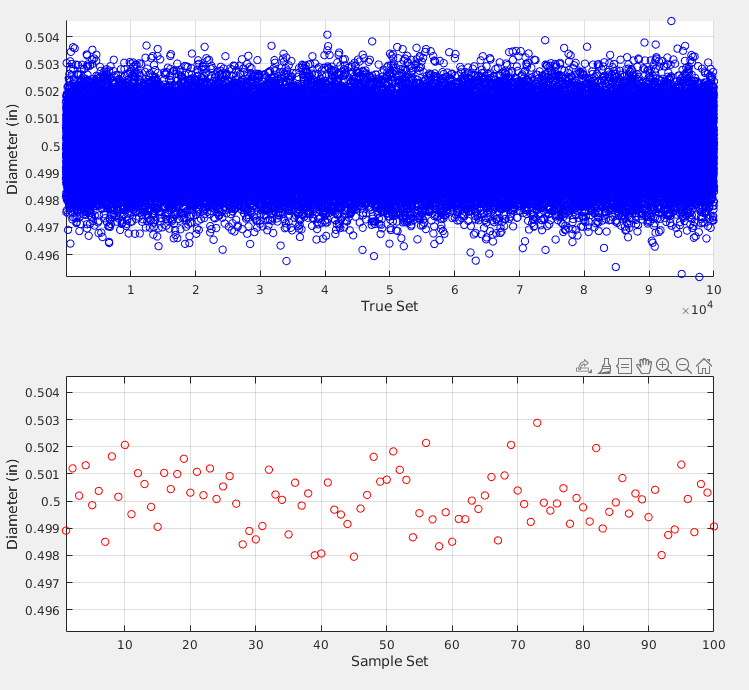
\includegraphics[scale=.20]{topic4_fig1.png}		
		
		\end{multicols}
		
	\end{frame}
	
%	% Section II - Frame II
%	\begin{frame} \small
%		\frametitle{\sectiontitleII}    
%		
%		
%	\end{frame}


\section{\sectiontitleIII}	

	% Section III - Frame I
	\begin{frame}[label=sectionIII] \small
		\frametitle{\sectiontitleIII}    
		
		We use a similar set of statistical parameters to describe the population after the true population has been sampled.
		
		\begin{multicols}{2} \tiny
		The sample mean is:\\
		\[ \bar{x}=\sum\limits_{i=1}^{N}x_i \]
		The sample variance and sample standard deviation:\\
		\[ s_x^2=\frac{1}{N-1}\sum\limits_{i=1}^{N}\left(x_i-\bar{x}\right)^2 \]
		The square root of the {\bf \BL sample variance} \\
		is the {\bf \PR sample standard deviation}. \\
		\[s_x=\sqrt{s_x^2}=\sqrt{\frac{1}{N-1}\sum\limits_{i=1}^{N}\left(x_i-\bar{x}\right)^2}\]

		\hspace*{0cm}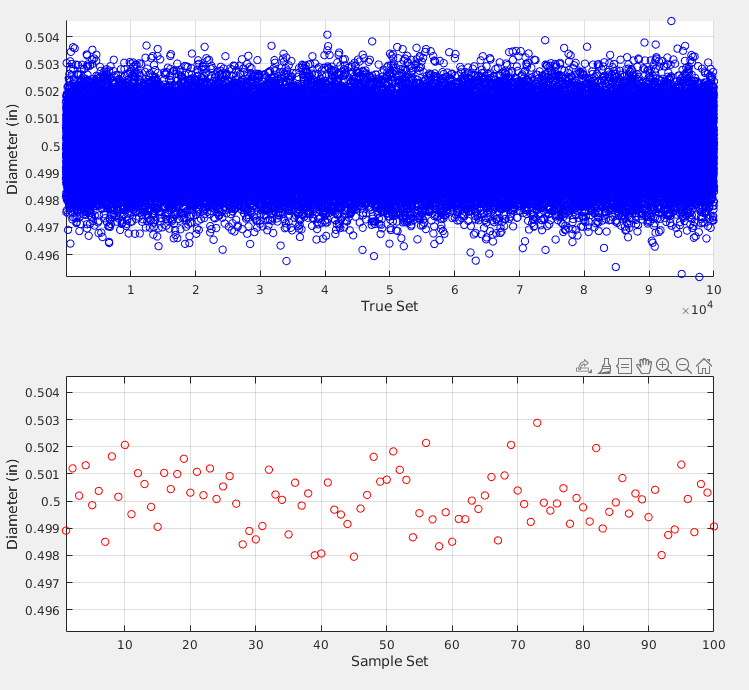
\includegraphics[scale=.20]{topic4_fig1.png}		
		
		\end{multicols}

	\end{frame}
	
	% Section III - Frame II
	\begin{frame} \scriptsize
		\frametitle{\sectiontitleIII}    
		
		The sample mean value provides a most probable estimate of the true mean value, $x'$. The sample variance represents a probable measure of the
variation found in a data set. The degrees of freedom, $n$, in a statistical estimate equate to the number
of data points minus the number of previously determined statistical parameters used in estimating
that value. For example, the degrees of freedom in the sample variance is $\nu = N - 1$, as seen in
denominator of Equations 4.14b and c. These equations are robust and are used regardless of the
actual probability density function of the measurand.
		
		
	\end{frame}
	
		% Section III - Frame II
	\begin{frame} \scriptsize
		\frametitle{\sectiontitleIII}    
		
		The relation between probability and infinite statistics can be extended to data sets of finite
sample size with only some modification. When data sets are finite or smaller than the population,
the $z$ variable does not provide a reliable weight estimate of the true probability. However, the
sample variance can be weighted in a similar manner so as to compensate for the difference between
the finite statistical estimates and the statistics based on an assumed $p(x)$. For a normal distribution
of $x$ about some sample mean value, $x$, we can state that statistically

\[x_i=\bar{x}\pm t_{\nu,P}s_x \hspace{3mm} P(\%)\]

where the variable t n,P provides a coverage factor used for finite data sets and which replaces the z
variable. This new variable is referred to as the Student’s t variable,

\[t=\frac{\bar{x}-x'}{s_x/\sqrt{N}} \]
		
		The interval $\pm t_{\nu,P}s_x$ represents a precision interval, given at probability $P\%$, within which one
should expect any measured value to fall.
		
	\end{frame}


\section{\sectiontitleIV}	
	% Section IV - Frame I
	\begin{frame}[label=sectionIV] \small
		\frametitle{\sectiontitleIV}    

\hspace*{0cm}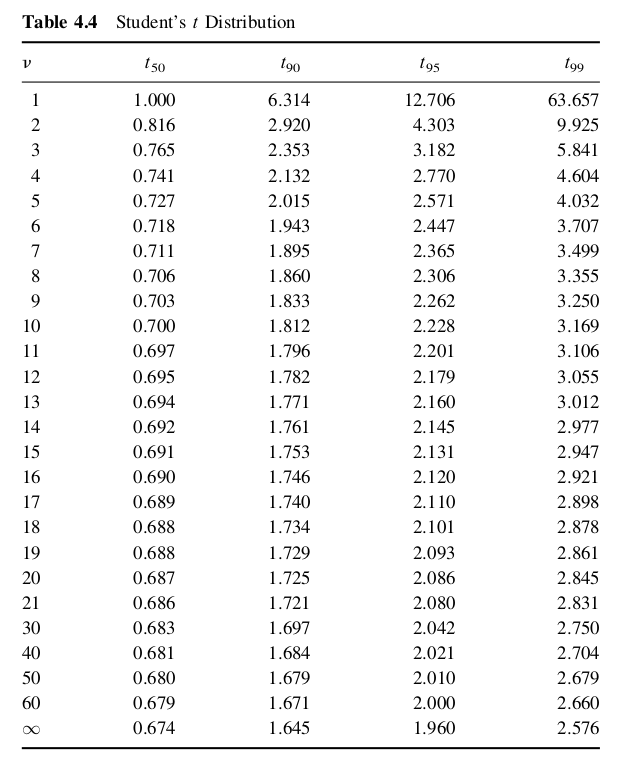
\includegraphics[scale=.25]{topic4_fig2.png}

	\end{frame}


\end{document}




	





